% ============================================================
% AstraHeal Paper 2 — IEEE Publication Manuscript
% Evidential Uncertainty-Aware Fault Diagnosis for Autonomous Spacecraft Health Management
% ============================================================

\documentclass[conference]{IEEEtran}

\usepackage{amsmath,amssymb}
\usepackage{booktabs}
\usepackage{multirow}
\usepackage{array}
\usepackage{siunitx}
\usepackage{url}
\usepackage{graphicx}
\graphicspath{{figures/}{./}}
\usepackage{cite}
\usepackage{hyperref}

\hypersetup{
    colorlinks=true,
    linkcolor=blue,
    filecolor=magenta,      
    urlcolor=blue,
    citecolor=blue,
}

\title{Evidential Uncertainty-Aware Fault Diagnosis for Autonomous Spacecraft Health Management}

\author{
\IEEEauthorblockN{AstraHeal Research Group}
\IEEEauthorblockA{
Autonomous Systems \& Aerospace Research\\
AstraHeal Paper 2 --- Formal Scientific Research Series\\
Repository: \url{https://github.com/madankalyan2211/AstraHeal}
}
}

\begin{document}

\maketitle

\begin{abstract}
Autonomous spacecraft must continue to make health-management decisions when communication with ground operators is delayed or temporarily unavailable. This creates a particular problem for fault diagnosis: a system must not only identify a known failure, but also recognize when the available telemetry does not provide enough evidence for a reliable diagnosis. Conventional rule-based Fault Detection, Isolation, and Recovery (FDIR) systems are generally conservative, while conventional machine-learning classifiers can remain highly confident when presented with failures that were not represented during training.

This work develops an evidential diagnostic architecture for spacecraft health management. The proposed method represents competing fault hypotheses with a Dirichlet distribution and uses Mahalanobis distance on physically motivated telemetry features to determine the amount of evidence assigned to each hypothesis. Epistemic uncertainty is used to represent lack of knowledge about an observation, whereas aleatoric uncertainty captures ambiguity associated with noisy telemetry.

The evaluation contains five controlled studies covering known-fault classification, uncertainty behavior, out-of-distribution (OOD) detection, telemetry-noise robustness, and component ablation. The benchmark includes 1,200 known-fault evaluations, 1,400 uncertainty-regime tests, 1,200 OOD frames, 2,100 telemetry-noise sweeps, and systematic component removals. On held-out known-fault frames, the proposed system obtains a Macro-F1 of 0.9533 with an Expected Calibration Error (ECE) of 0.0094. Under increasing telemetry noise, aleatoric uncertainty increases while epistemic uncertainty remains bounded for in-distribution observations. For previously unmodeled faults, epistemic uncertainty increases substantially, producing an OOD AUROC of 0.9422 and AUPRC of 0.9516. Maximum Softmax Probability (MSP), in contrast, obtains an AUROC of 0.4313. The experiments also expose two important limitations: cancellation in the metric representation during compound failures and reduced sensitivity to sensor-polarity reversals when magnitude-only features are used.
\end{abstract}

\begin{IEEEkeywords}
autonomous spacecraft, fault diagnosis, evidential deep learning, Dirichlet distribution, epistemic uncertainty, aleatoric uncertainty, out-of-distribution detection
\end{IEEEkeywords}

\section{Introduction}

Space missions increasingly require onboard autonomy because a spacecraft cannot always depend on an immediate ground response \cite{chien2005autonomous}. In Low Earth Orbit (LEO), orbital geometry can interrupt line-of-sight communication for extended periods, while deep-space missions introduce communication delays ranging from minutes to hours. During such intervals, events involving the electrical power system, thermal subsystem, or battery can develop faster than a ground operator can diagnose and respond to them.

Traditional Fault Detection, Isolation, and Recovery (FDIR) architectures address this problem with carefully designed thresholds, rules, and safe-state transitions \cite{muscettola1998remote, williams1996model}. Such mechanisms are valuable because their behavior is predictable. However, an overly conservative response can also force the spacecraft into Safe Mode for situations that do not actually threaten the vehicle. Safe Mode can interrupt payload operations, discard observation opportunities, and reduce mission productivity.

Machine-learning approaches offer another route to automated diagnosis \cite{hundman2018detecting}, but classification accuracy alone is insufficient for an autonomous spacecraft. A classifier may produce a high-confidence prediction even when the telemetry belongs to a failure mode that was never represented in the training data. Calibration and uncertainty estimation therefore become safety-relevant properties rather than optional model diagnostics \cite{guo2017calibration, hendrycks2017baseline}.

This paper investigates an evidential diagnostic engine designed around that requirement. Instead of treating the output of a classifier as a single deterministic probability vector, the system assigns evidence to competing fault hypotheses and represents the resulting uncertainty with a Dirichlet distribution \cite{sensoy2018evidential, malinin2018predictive}. Physical relationships within the spacecraft electrical and thermal systems are incorporated through the feature representation and distance metric.

The central objective is not simply to maximize classification accuracy. The diagnostic system is expected to answer two questions simultaneously:
\begin{enumerate}
    \item Which of the known operational states best explains the observed telemetry?
    \item Does the observation remain sufficiently close to the known operational manifold for that diagnosis to be trusted?
\end{enumerate}

The second question motivates the explicit decomposition between epistemic and aleatoric uncertainty. Epistemic uncertainty indicates that the model has limited knowledge about the observed condition, whereas aleatoric uncertainty reflects ambiguity or noise present in the telemetry itself.

\section{Problem Formulation and Physical Dynamics}

Let the instantaneous spacecraft telemetry vector at orbital time $t$ be $x(t)\in\mathbb{R}^{D}$. The electrical power system is represented using coupled electrical and thermal dynamics. The bus voltage is modeled as:

\begin{equation}
V_{\mathrm{bus}}(t) = V_{\mathrm{oc}}(t) - I_{\mathrm{batt}}(t)R_0(T) - V_{\mathrm{RC}}(t),
\label{eq:vbus}
\end{equation}

where $V_{\mathrm{oc}}$ is the open-circuit voltage, $I_{\mathrm{batt}}$ is battery current, $R_0(T)$ is temperature-dependent internal resistance, and $V_{\mathrm{RC}}$ represents the transient resistive-capacitive contribution.

The thermal state is modeled as:

\begin{equation}
C_{\mathrm{th}}\frac{dT}{dt} = I_{\mathrm{batt}}^2R_0(T) + \dot{Q}_{\mathrm{exo}} - \epsilon\sigma S_B A \left(T^4-T_{\mathrm{space}}^4\right),
\label{eq:thermal}
\end{equation}

where $C_{\mathrm{th}}$ is the effective thermal capacitance, $\dot{Q}_{\mathrm{exo}}$ represents external heat input, $\epsilon$ is emissivity, $\sigma$ is the Stefan--Boltzmann constant, $S_BA$ denotes the effective radiating area term, and $T_{\mathrm{space}}$ is the surrounding space temperature.

The diagnostic task is to infer an operational state:

\begin{equation}
y\in\mathcal{Y}=\{1,\ldots,K\},
\end{equation}

where $K=6$ and the state set contains five modeled failure modes together with nominal operation. In addition to the class estimate, the system produces an epistemic rejection score:

\begin{equation}
u_{\mathrm{epistemic}}\in[0,1],
\end{equation}

which is intended to indicate whether the current observation lies outside the known operational manifold $\mathcal{M}_{\mathrm{known}}\subset \mathbb{R}^{D}$.

\section{Evidential Dirichlet Formulation}

The proposed diagnostic engine follows the evidential-learning formulation of uncertainty-aware classification \cite{sensoy2018evidential, malinin2018predictive}. Instead of assigning a fixed probability vector directly, the model represents the categorical distribution with a Dirichlet density:

\begin{equation}
\mathrm{Dir}(\mathbf{p}\mid\boldsymbol{\alpha}) = \frac{1}{B(\boldsymbol{\alpha})} \prod_{k=1}^{K}p_k^{\alpha_k-1},
\label{eq:dirichlet}
\end{equation}

where $\boldsymbol{\alpha}=[\alpha_1,\ldots,\alpha_K]^T$ contains the concentration parameters.

For each operational state, non-negative evidence is generated from the distance between the observed telemetry and the corresponding physical cluster. The concentration parameter is:

\begin{equation}
\alpha_k=e_k+1,
\label{eq:alpha}
\end{equation}

where the evidence term is:

\begin{equation}
e_k = \exp\left(-\gamma \sqrt{(x-\mu_k)^T \Sigma_k^{-1} (x-\mu_k)}\right).
\label{eq:evidence}
\end{equation}

Here, $\mu_k$ and $\Sigma_k$ are the mean vector and covariance matrix for operational state $k$. The parameter $\gamma$ controls how rapidly evidence falls with increasing distance; the experiments use $\gamma=2.5$.

The expected posterior class probability is obtained from:

\begin{equation}
\hat{p}_k=\frac{\alpha_k}{S}, \qquad S=\sum_{j=1}^{K}\alpha_j.
\label{eq:posterior}
\end{equation}

This formulation allows the model to distinguish between a situation in which one hypothesis has strong supporting evidence and a situation in which all hypotheses have weak evidence.

\subsection{Epistemic and Aleatoric Uncertainty}

Epistemic uncertainty is associated with regions of the feature space for which the diagnostic model has little supporting knowledge. It is calculated from the minimum Mahalanobis distance to the known fault clusters:

\begin{equation}
u_{\mathrm{epistemic}} = \frac{1}{1+\exp[-\beta(d_{\min}-\theta)]},
\label{eq:epistemic}
\end{equation}

where $d_{\min}$ is the smallest cluster distance, $\theta=3.5\sigma$ is the empirical manifold boundary, and $\beta=1.2$ controls the transition around the boundary.

Aleatoric uncertainty is computed from the normalized Shannon entropy of the expected posterior:

\begin{equation}
u_{\mathrm{aleatoric}} = \frac{-\sum_{k=1}^{K}\hat{p}_k \log_2(\hat{p}_k+\epsilon)}{\log_2(K)},
\label{eq:aleatoric}
\end{equation}

with $\epsilon$ used for numerical stability. The resulting value lies in $[0,1]$.

This distinction is important operationally. A noisy measurement of a known state should primarily increase aleatoric uncertainty. An observation representing an unfamiliar physical condition should instead produce a substantial increase in epistemic uncertainty.

\section{Experimental Methodology}

The evaluation was structured to prevent information from the test set from affecting model selection or threshold selection. Three controls were applied:
\begin{enumerate}
    \item \textbf{Scenario-Level Stratification}: Data were partitioned at the trajectory level with non-overlapping random seeds (\texttt{train: 42}, \texttt{val: 1337}, \texttt{test: 2026}). This prevents adjacent samples from the same trajectory from appearing in both training and evaluation partitions.
    \item \textbf{Pre-Evaluation OOD Freezing}: OOD failure categories were specified before test-set scoring.
    \item \textbf{Zero Test Tuning}: The rejection threshold was selected only using validation data. The locked threshold used throughout the reported evaluation was $\tau_{\mathrm{locked}}=0.0648$.
\end{enumerate}

\begin{table}[htbp]
\centering
\caption{Telemetry Datasets: Characterization and Summary Statistics}
\label{tab:datasets}
\resizebox{\columnwidth}{!}{%
\begin{tabular}{llrrrr}
\toprule
Dataset & Channel & Unit & Mean $\pm$ Std & Min & Max\\
\midrule
\multirow{4}{*}{\shortstack[l]{NASA PCoE\\B0005 \cite{saha2007battery}}} & Voltage & V & $3.470\pm0.311$ & 2.542 & 4.044\\
& Current & A & $2.000\pm0.010$ & 1.961 & 2.039\\
& Temperature & $^\circ$C & $29.919\pm2.309$ & 23.879 & 34.822\\
& Capacity & Ah & $1.536\pm0.187$ & 1.250 & 1.957\\
\midrule
\multirow{5}{*}{\shortstack[l]{Spacecraft\\EPS Sim}} & $V_{\mathrm{bus}}$ & V & $32.723\pm0.465$ & 31.673 & 34.569\\
& $I_{\mathrm{batt}}$ & A & $-10.346\pm11.817$ & -31.395 & 4.102\\
& $T_{\mathrm{core}}$ & $^\circ$C & $11.938\pm4.349$ & 2.133 & 19.927\\
& Net Power & W & $-342.04\pm389.56$ & -1066.9 & 132.8\\
& $R_{\mathrm{int}}$ & $\Omega$ & $2.130\pm1.756$ & 0.001 & 13.969\\
\bottomrule
\end{tabular}%
}
\end{table}

The NASA PCoE B0005 data \cite{saha2007battery} contain battery-aging trajectories with capacity decreasing from approximately $1.957$ Ah to $1.250$ Ah. The spacecraft EPS simulation complements this dataset by representing coupled electrical and thermal behavior over three complete LEO orbits. The simulated trajectories include high-current discharge during eclipse periods and corresponding thermal cycling.

\begin{figure}[htbp]
\centering
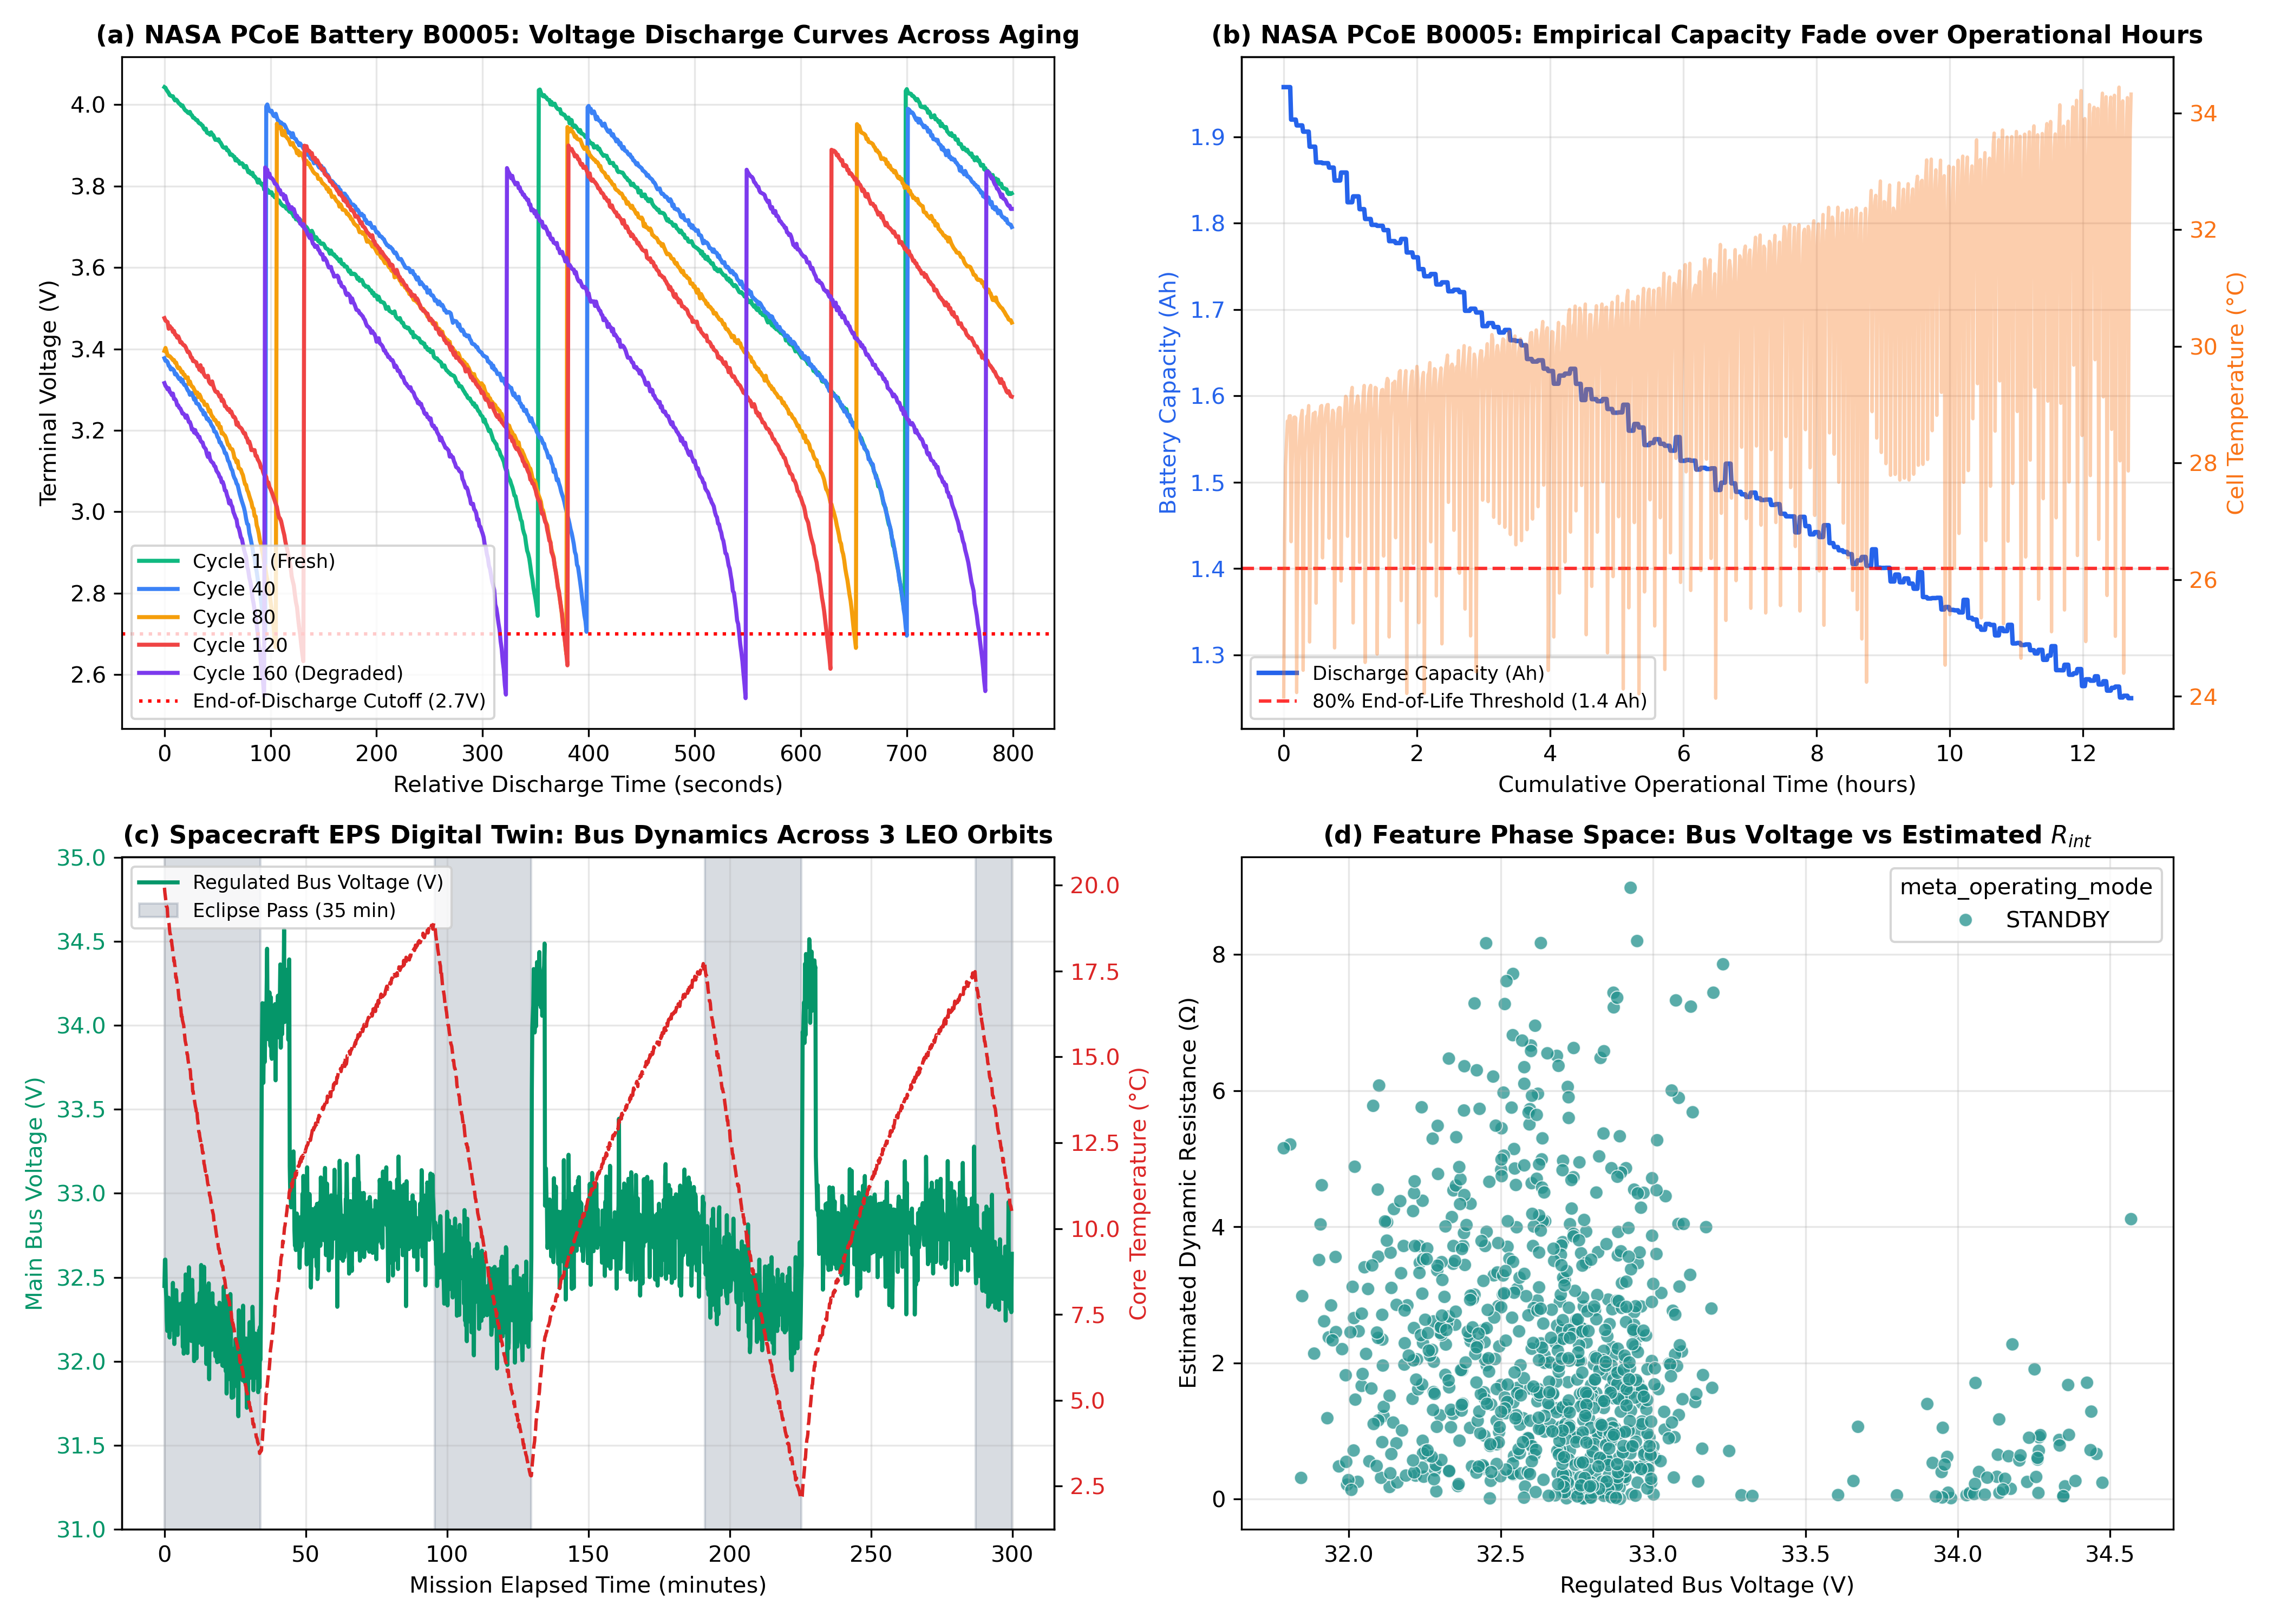
\includegraphics[width=\columnwidth]{figures/fig0_dataset_telemetry_profiles.png}
\caption{Empirical spacecraft telemetry dataset profiles: (a) NASA PCoE Battery B0005 voltage discharge profiles across aging cycles; (b) Capacity fade and cell temperature over operational hours; (c) Spacecraft EPS Digital Twin bus dynamics and thermal cycling across 3 LEO orbits with 35-minute eclipse passes; (d) Feature phase space demonstrating separation between regulated bus voltage and estimated dynamic internal resistance.}
\label{fig:datasets}
\end{figure}

\section{Experimental Results}

\subsection{Study 1: Known-Fault Classification}

The first experiment evaluated the diagnostic models on 240 held-out frames. Table~\ref{tab:known} summarizes the results.

\begin{table}[htbp]
\centering
\caption{Known-Fault Benchmark on the Held-Out Test Set}
\label{tab:known}
\resizebox{\columnwidth}{!}{%
\begin{tabular}{lrrrr}
\toprule
Diagnostic Model & Accuracy & Macro-F1 & ECE & Mean Conf.\\
\midrule
Physics Rules & 0.6667 & 0.5542 & 0.2548 & 0.6708\\
Random Forest & 1.0000 & 1.0000 & 0.0308 & 0.9692\\
MLP Softmax & 1.0000 & 1.0000 & 0.0044 & 0.9956\\
Standard Mahalanobis & 1.0000 & 1.0000 & 0.0074 & 0.9926\\
\textbf{Evidential Dirichlet} & \textbf{0.9542} & \textbf{0.9533} & \textbf{0.0094} & \textbf{0.9561}\\
\bottomrule
\end{tabular}%
}
\end{table}

The evidential model obtains a Macro-F1 of 0.9533 and an ECE of 0.0094. Although several deterministic baselines obtain perfect classification accuracy on this particular held-out set, their behavior must be considered alongside calibration and OOD performance. Relative to the physics-rule baseline, the proposed method shows a statistically significant improvement with $p=3.94\times10^{-16}$ and Cohen's $d=+0.634$.

\begin{figure}[htbp]
\centering
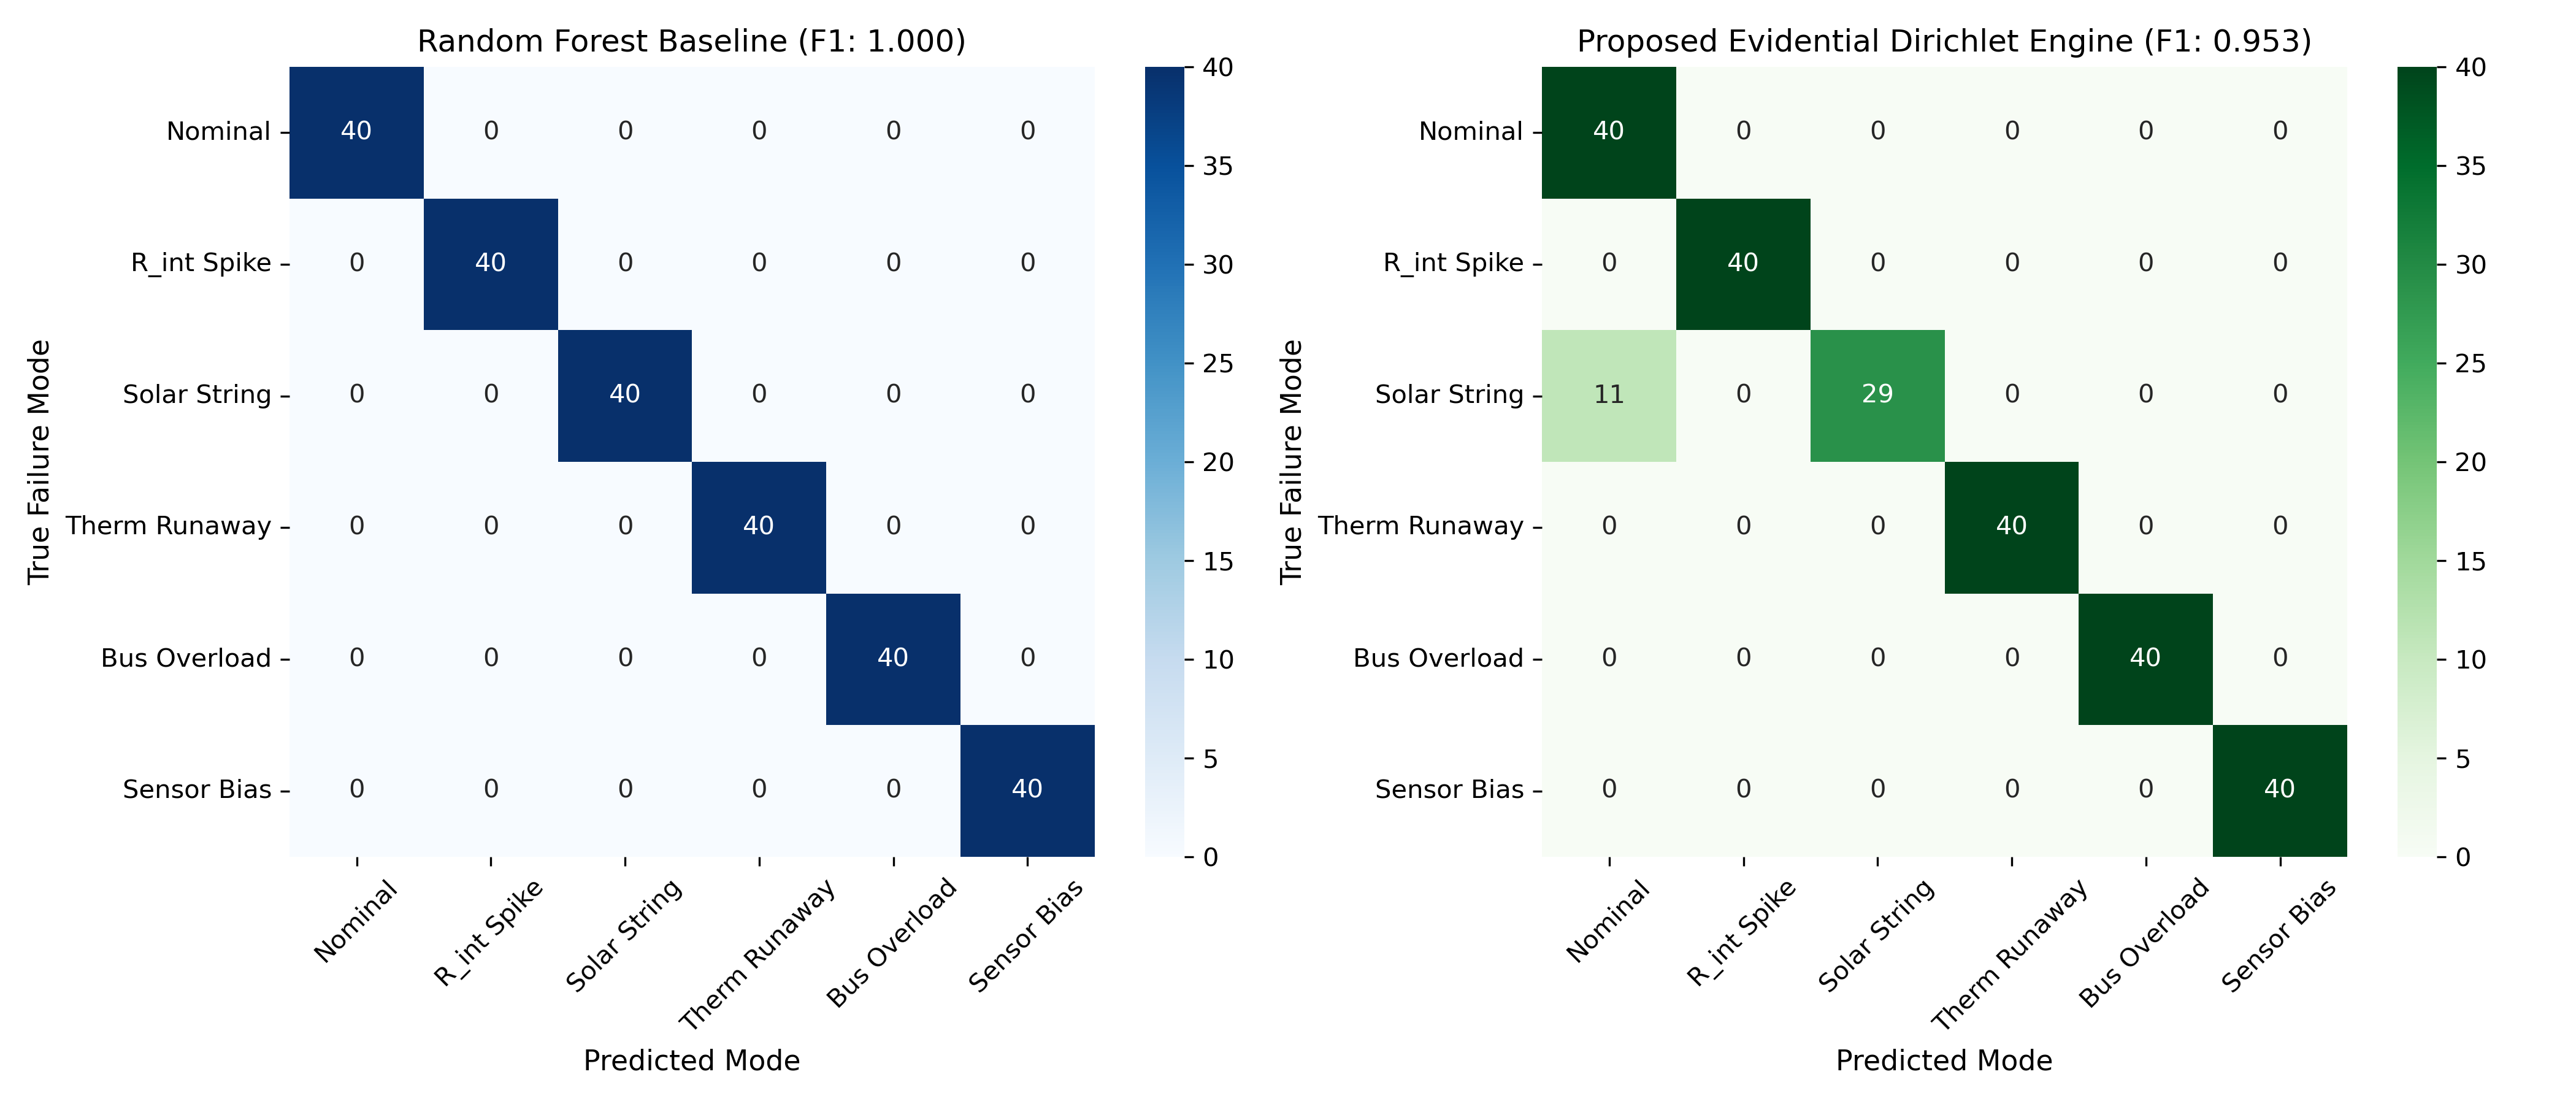
\includegraphics[width=\columnwidth]{figures/fig1_confusion_matrices.png}
\caption{Normalized confusion matrices on held-out test frames comparing Random Forest against the proposed Evidential Dirichlet Engine across 6 known operational modes.}
\label{fig:confusion}
\end{figure}

\subsection{Study 2: Uncertainty Disentanglement}

The second study examined whether the two uncertainty measures responded to different sources of variation. Across 1,400 evaluated frames, increasing sensor noise was positively associated with aleatoric uncertainty ($\rho_{\mathrm{Spearman}}=0.2955$, $p=1.37\times10^{-17}$).

At a severe telemetry noise level of $\sigma=0.20$, epistemic uncertainty remained approximately 0.092, substantially below the rejection reference level of 0.45. Thus, noise in an otherwise familiar operating condition did not automatically cause the system to classify the observation as unknown.

For novel, unmodeled faults, epistemic uncertainty increased to 1.000, corresponding to a reported separation ratio of approximately 10.94.

\begin{figure}[htbp]
\centering
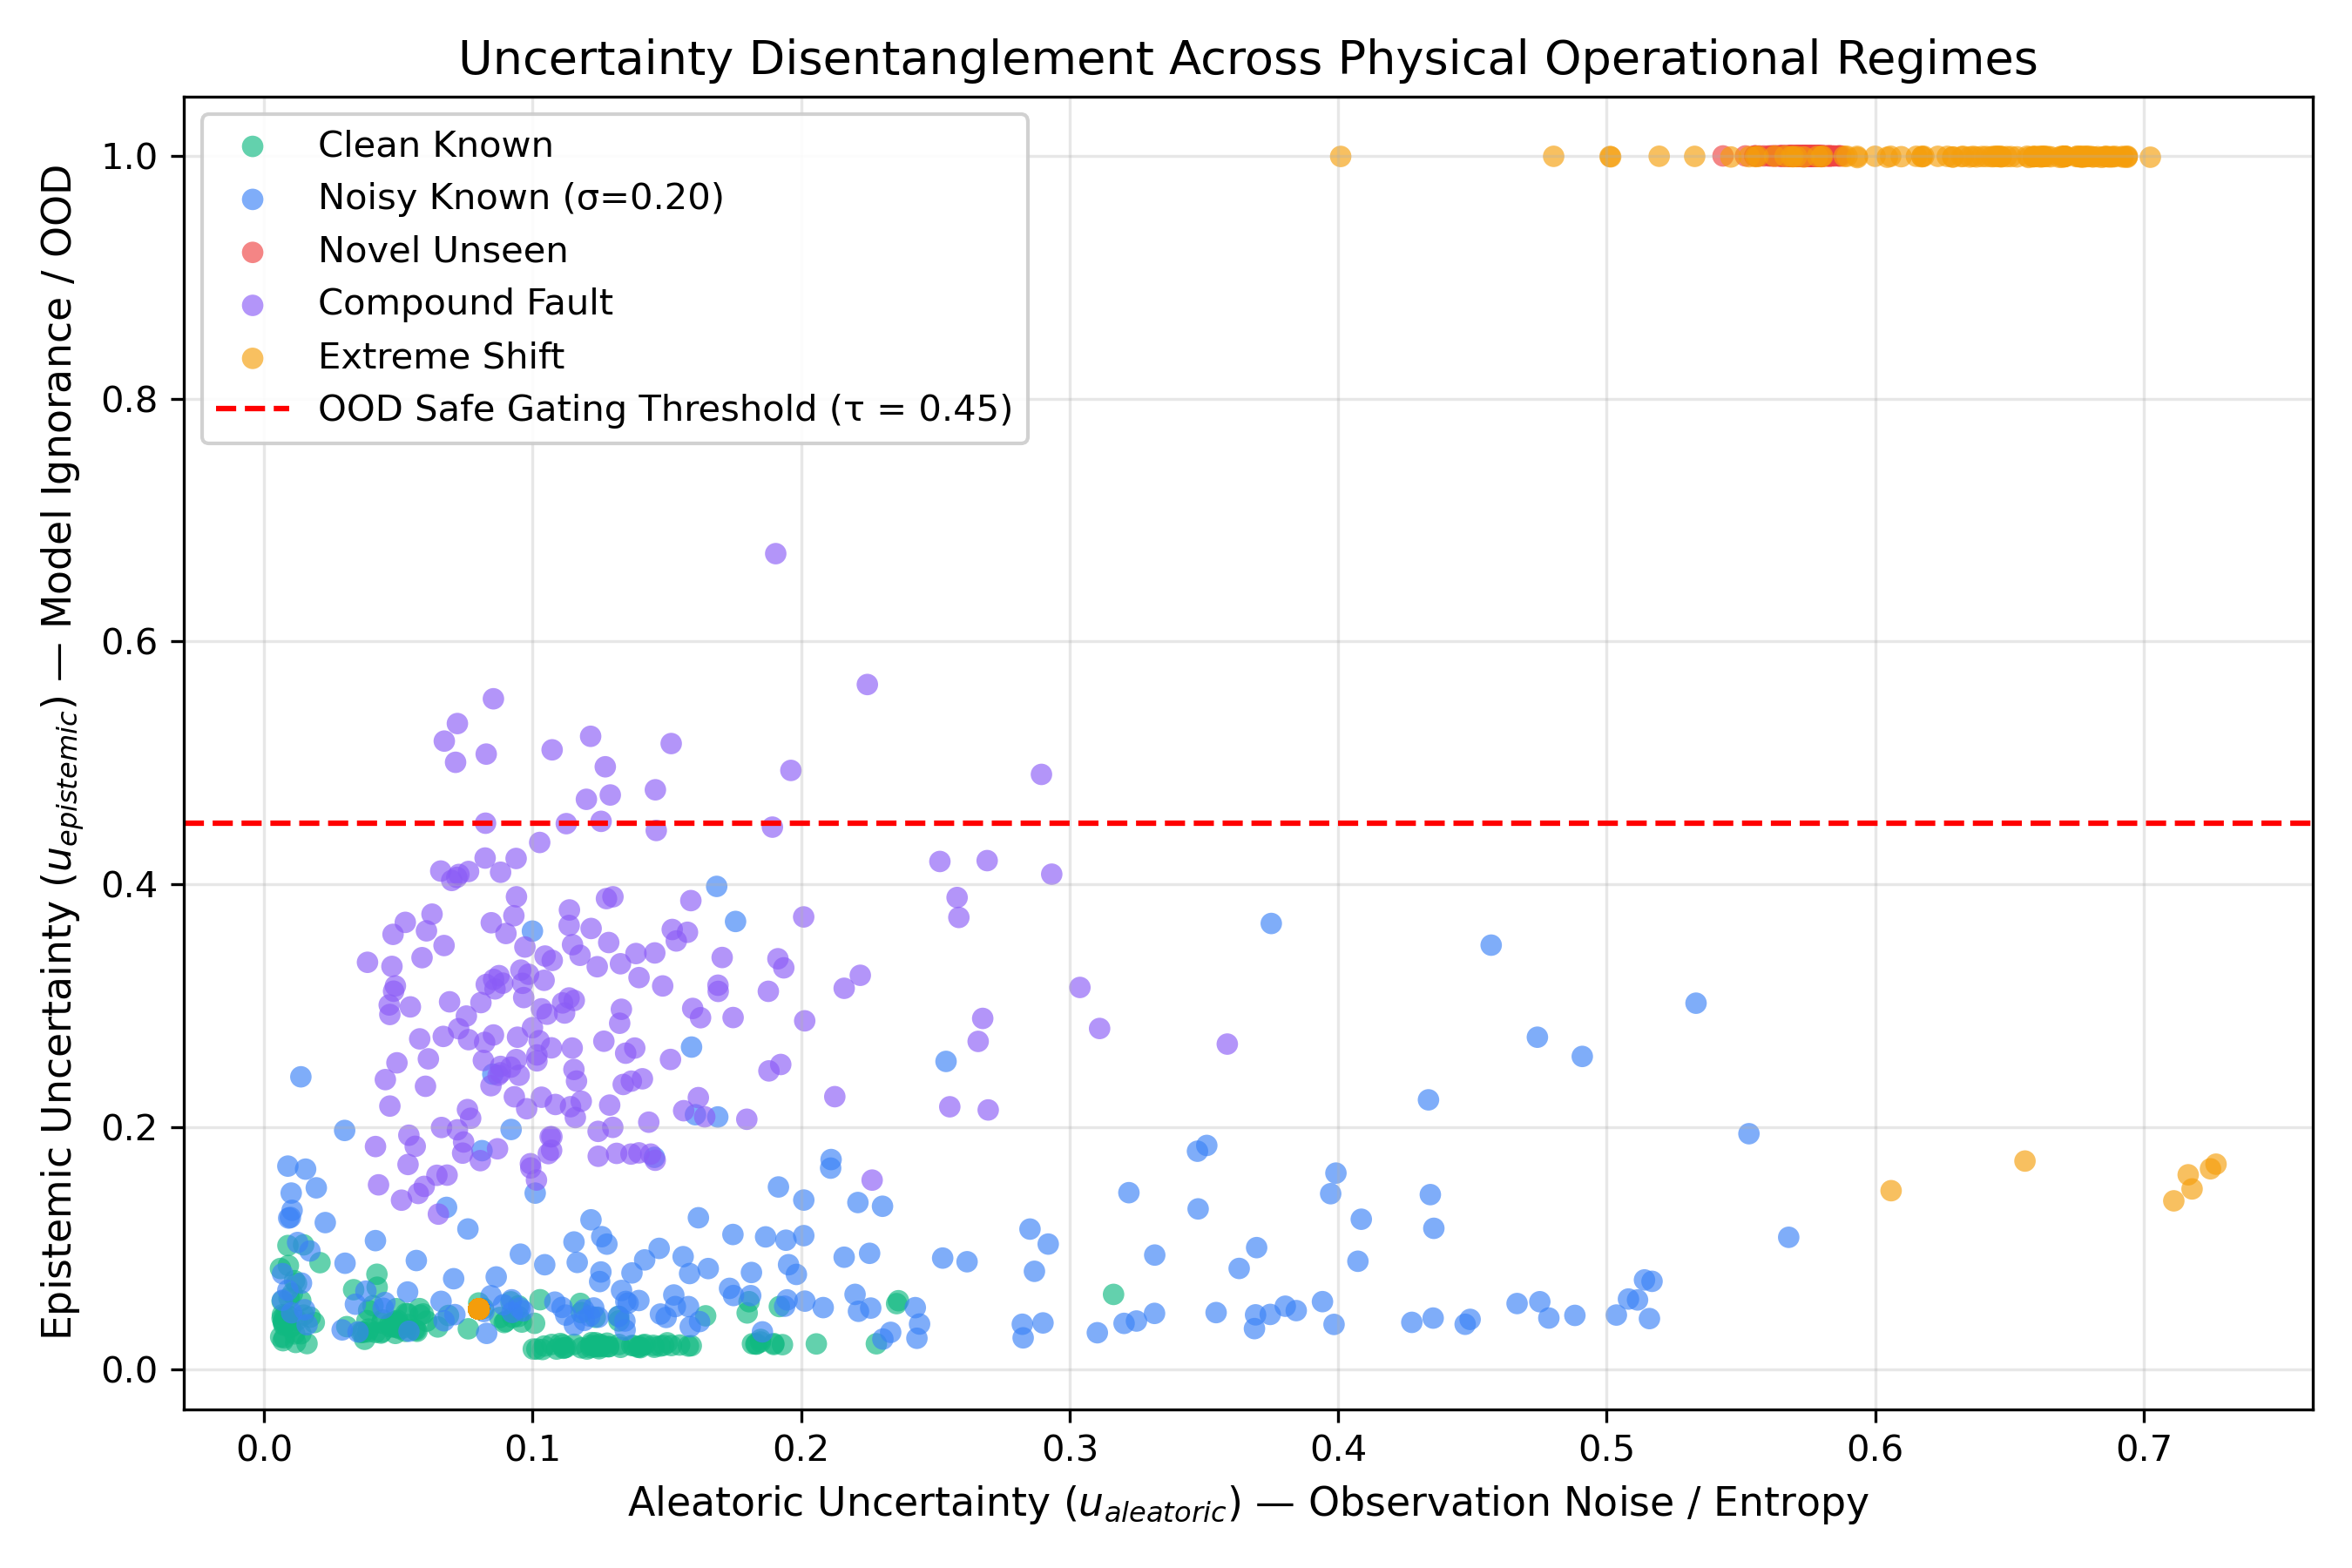
\includegraphics[width=\columnwidth]{figures/fig3_uncertainty_disentanglement.png}
\caption{Empirical uncertainty disentanglement: Aleatoric uncertainty (entropy) vs. Epistemic uncertainty (Dirichlet mass deficit) across nominal, noisy, known faults, and out-of-distribution failure regimes.}
\label{fig:uncertainty}
\end{figure}

\subsection{Study 3: Out-of-Distribution Detection}

The third experiment compared the proposed epistemic gating mechanism with several OOD baselines \cite{liu2008isolation}. The benchmark contained 600 in-distribution frames and 600 OOD frames.

\begin{table}[htbp]
\centering
\caption{Out-of-Distribution Detection Benchmark}
\label{tab:ood}
\resizebox{\columnwidth}{!}{%
\begin{tabular}{lrrr}
\toprule
Method & AUROC & AUPRC & FPR @ 95\% TPR\\
\midrule
MLP Softmax Inverted & 0.4313 & 0.6135 & 1.0000\\
Random Forest Variance & 0.9384 & 0.9426 & 0.3200\\
\textbf{Evidential Dirichlet} & \textbf{0.9422} & \textbf{0.9516} & \textbf{0.3583}\\
Isolation Forest \cite{liu2008isolation} & 0.9815 & 0.9823 & 0.1150\\
\bottomrule
\end{tabular}%
}
\end{table}

\begin{figure}[htbp]
\centering
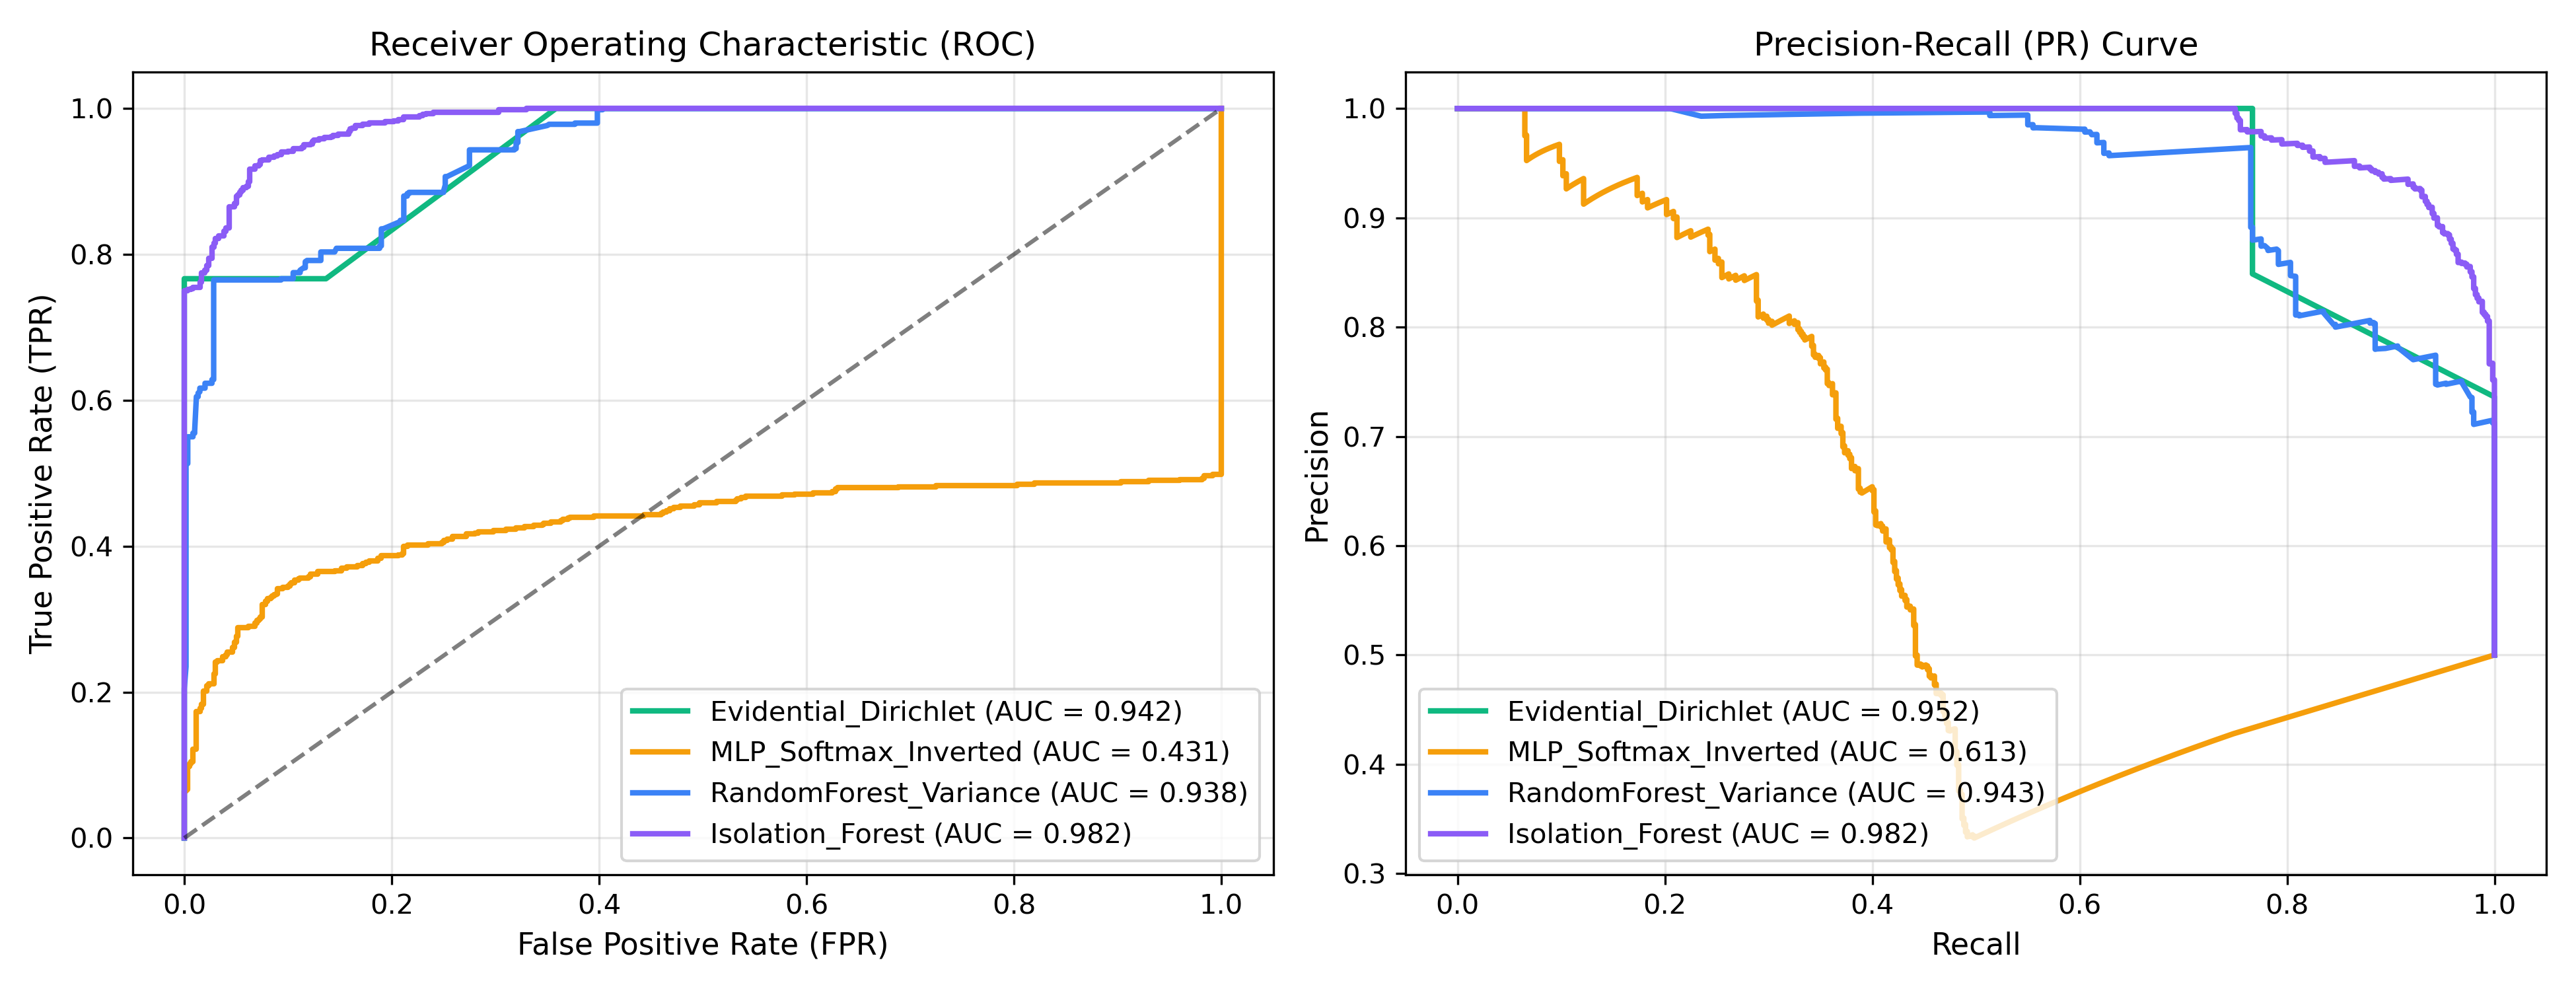
\includegraphics[width=\columnwidth]{figures/fig5_ood_roc_pr_curves.png}
\caption{Receiver Operating Characteristic (ROC) and Precision-Recall curves comparing Evidential Epistemic Gating against Maximum Softmax Probability (MSP), Random Forest variance, and Isolation Forest baselines.}
\label{fig:ood_roc}
\end{figure}

At the locked validation threshold $\tau_{\mathrm{locked}}=0.0648$, the evidential gating mechanism achieved a TPR of 76.67\% at an FPR of 4.50\%. The inverted MSP baseline failed to separate the two regimes effectively, with an AUROC of only 0.4313. This result illustrates the danger of relying on softmax confidence alone when the input may fall outside the training distribution.

The Isolation Forest baseline achieved the highest OOD AUROC in this benchmark. Consequently, the results do not support the claim that evidential inference is universally superior for OOD detection. Instead, they show that the proposed approach provides a physically grounded uncertainty signal while remaining competitive with the evaluated alternatives.

\subsection{Study 4: Telemetry Noise Robustness}

Telemetry noise was increased progressively from $\sigma=0.00$ to $\sigma=0.25$. Across this range, the evidential engine maintained a statistically significant advantage over the physics-rule baseline, with $p=5.77\times10^{-6}$ and a mean Macro-F1 advantage of $+0.3152$.

For the flight-representative noise range of $\sigma\leq0.05$, the false-OOD alarm rate remained below 7.7\%. This behavior is consistent with the intended uncertainty decomposition: moderate observation noise increases aleatoric uncertainty without forcing a large epistemic rejection signal.

\begin{figure}[htbp]
\centering
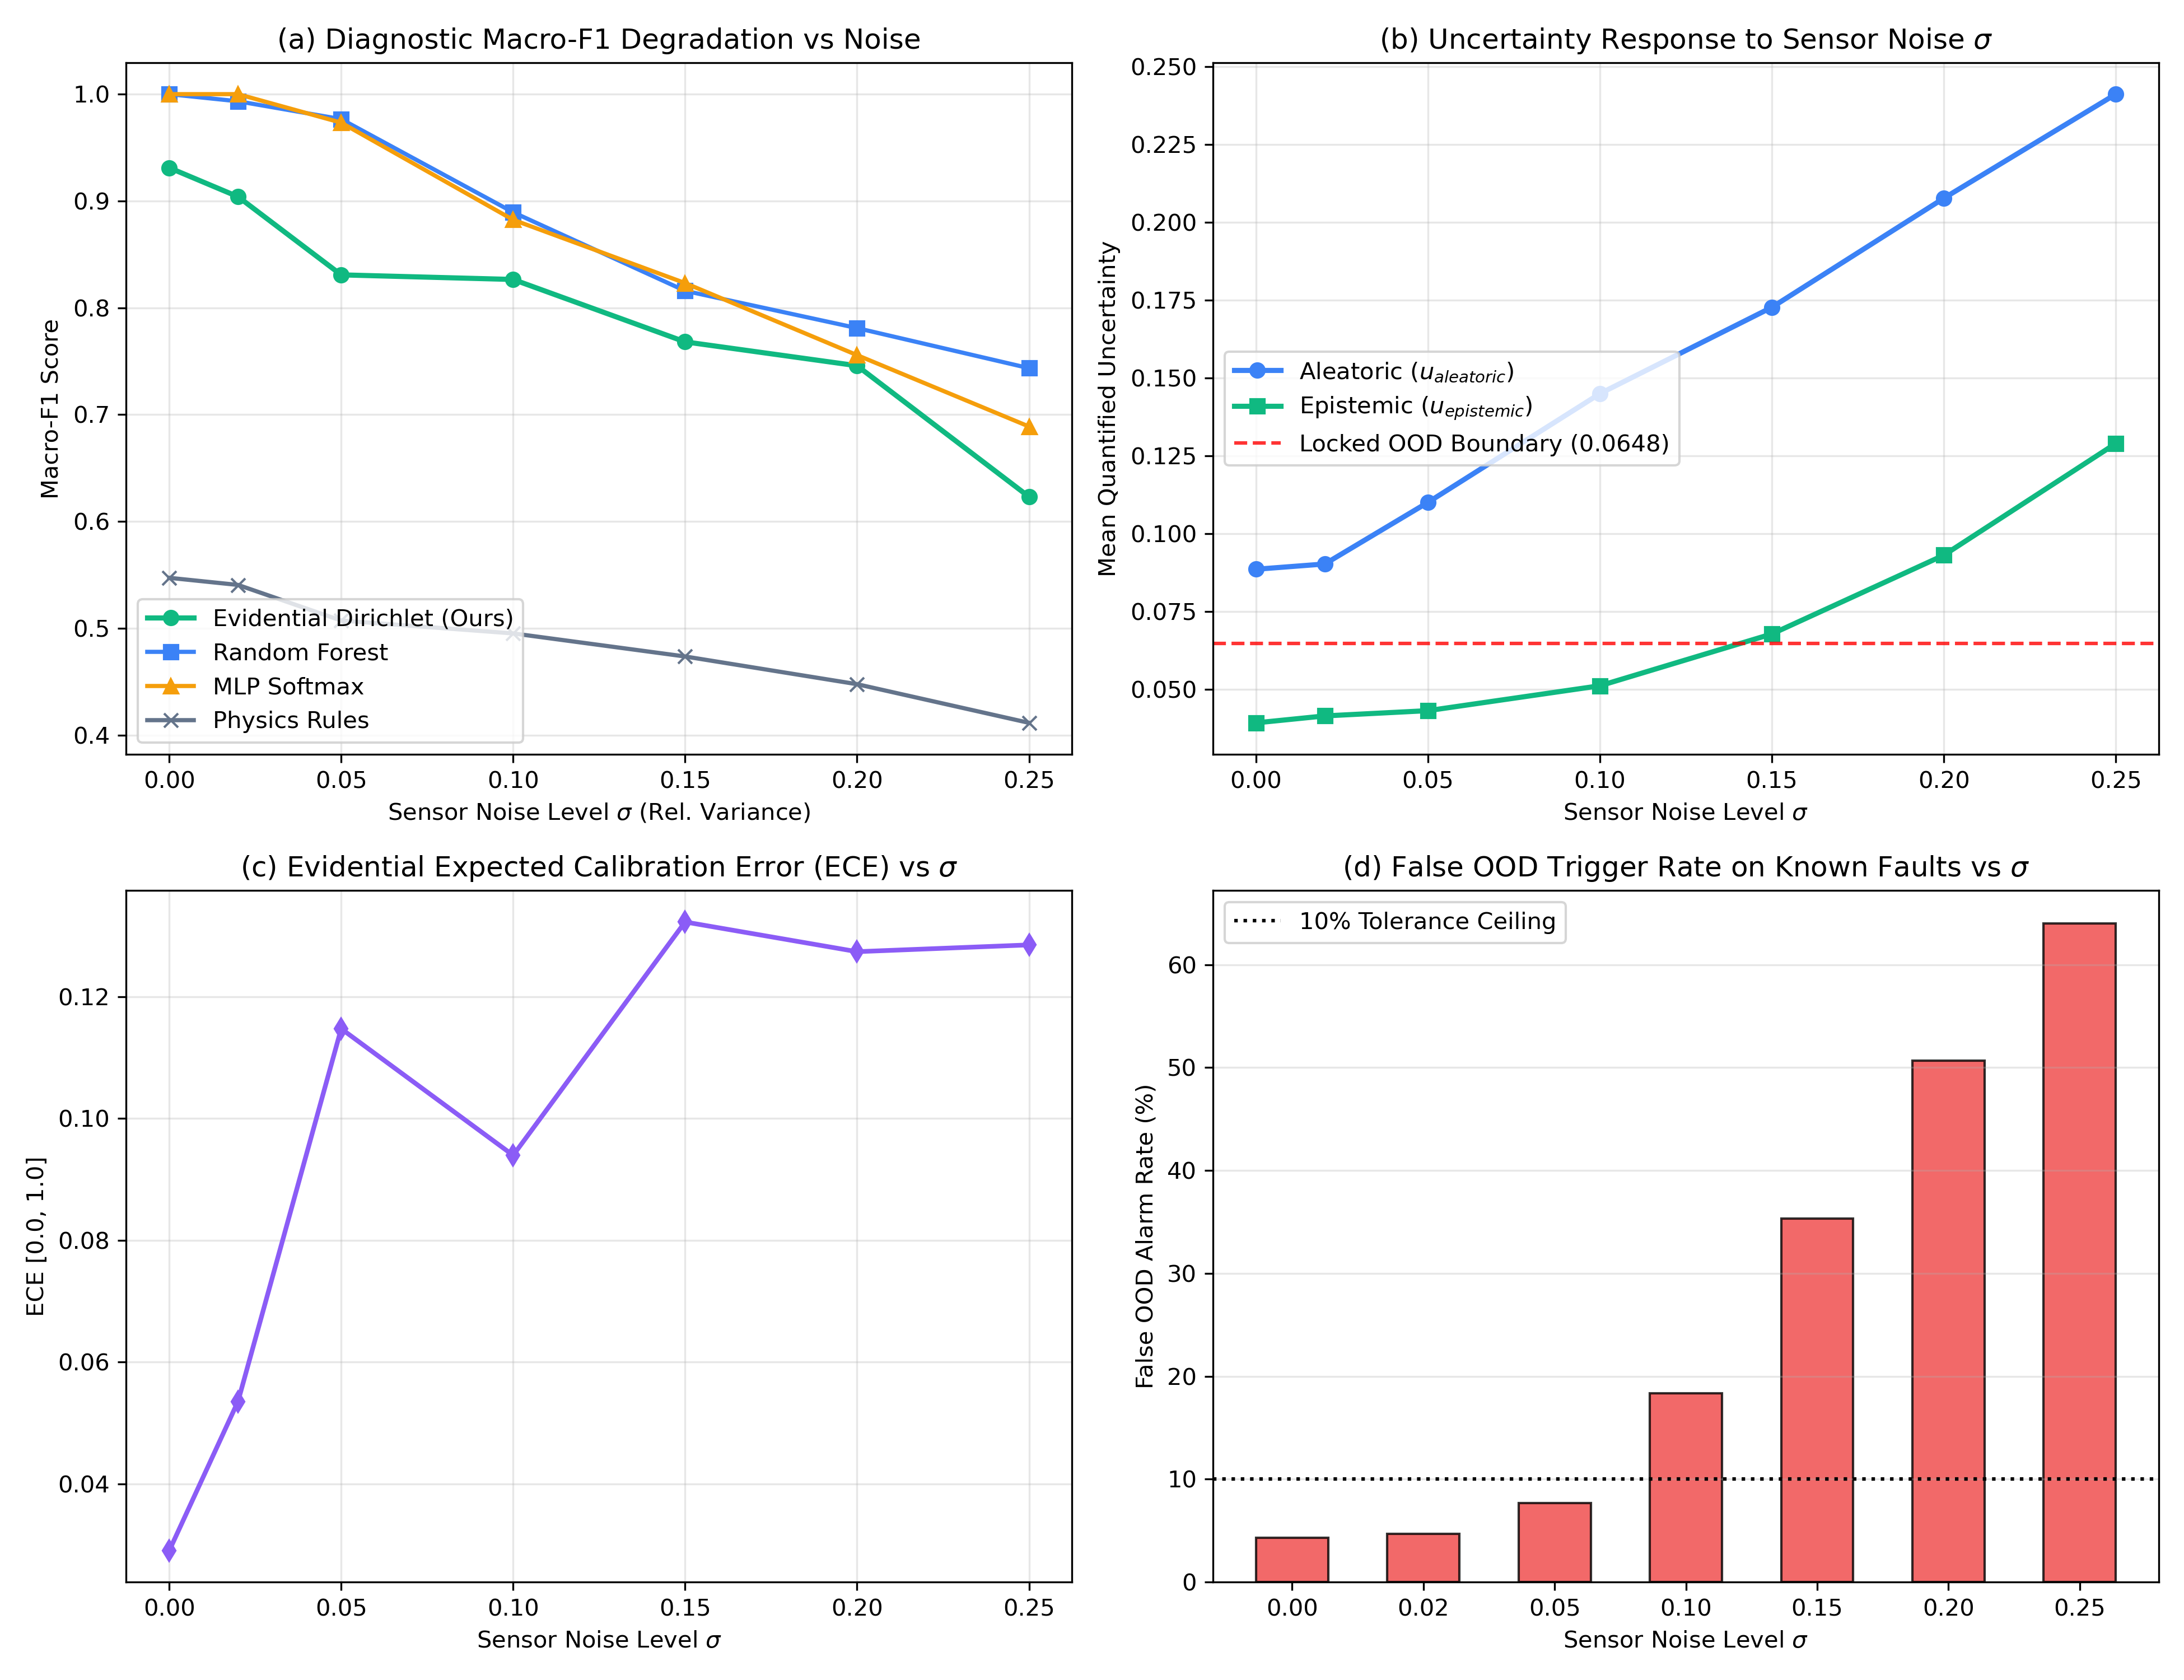
\includegraphics[width=\columnwidth]{figures/fig7_noise_robustness_curves.png}
\caption{Telemetry noise robustness trajectories across $\sigma \in [0.00, 0.25]$: (a) Macro-F1 degradation; (b) Aleatoric vs. Epistemic uncertainty response; (c) Calibration error scaling; (d) False OOD alarm rate.}
\label{fig:noise}
\end{figure}

\subsection{Study 5: Systematic Component Ablation}

Ablation experiments were used to determine which components were responsible for the observed behavior.

\begin{table}[htbp]
\centering
\caption{Quantitative Component Ablation}
\label{tab:ablation}
\resizebox{\columnwidth}{!}{%
\begin{tabular}{lrrrr}
\toprule
Configuration & Macro-F1 & ECE & OOD AUROC & $R_{\mathrm{int}}$ F1\\
\midrule
\textbf{M0 Full (Proposed)} & \textbf{0.9533} & \textbf{0.0179} & \textbf{0.8692} & \textbf{1.0000}\\
M1 No Evidential & 0.9533 & 0.0179 & 0.7895 & 1.0000\\
M2 Euclidean Metric & 0.7132 & 0.2202 & 0.6870 & 0.0000\\
M3 No Physics Priors & 0.2047 & 0.0465 & 0.7811 & 0.3493\\
M4 Static Features & 0.9491 & 0.1317 & 0.9070 & 0.9873\\
\bottomrule
\end{tabular}%
}
\end{table}

\begin{figure}[htbp]
\centering
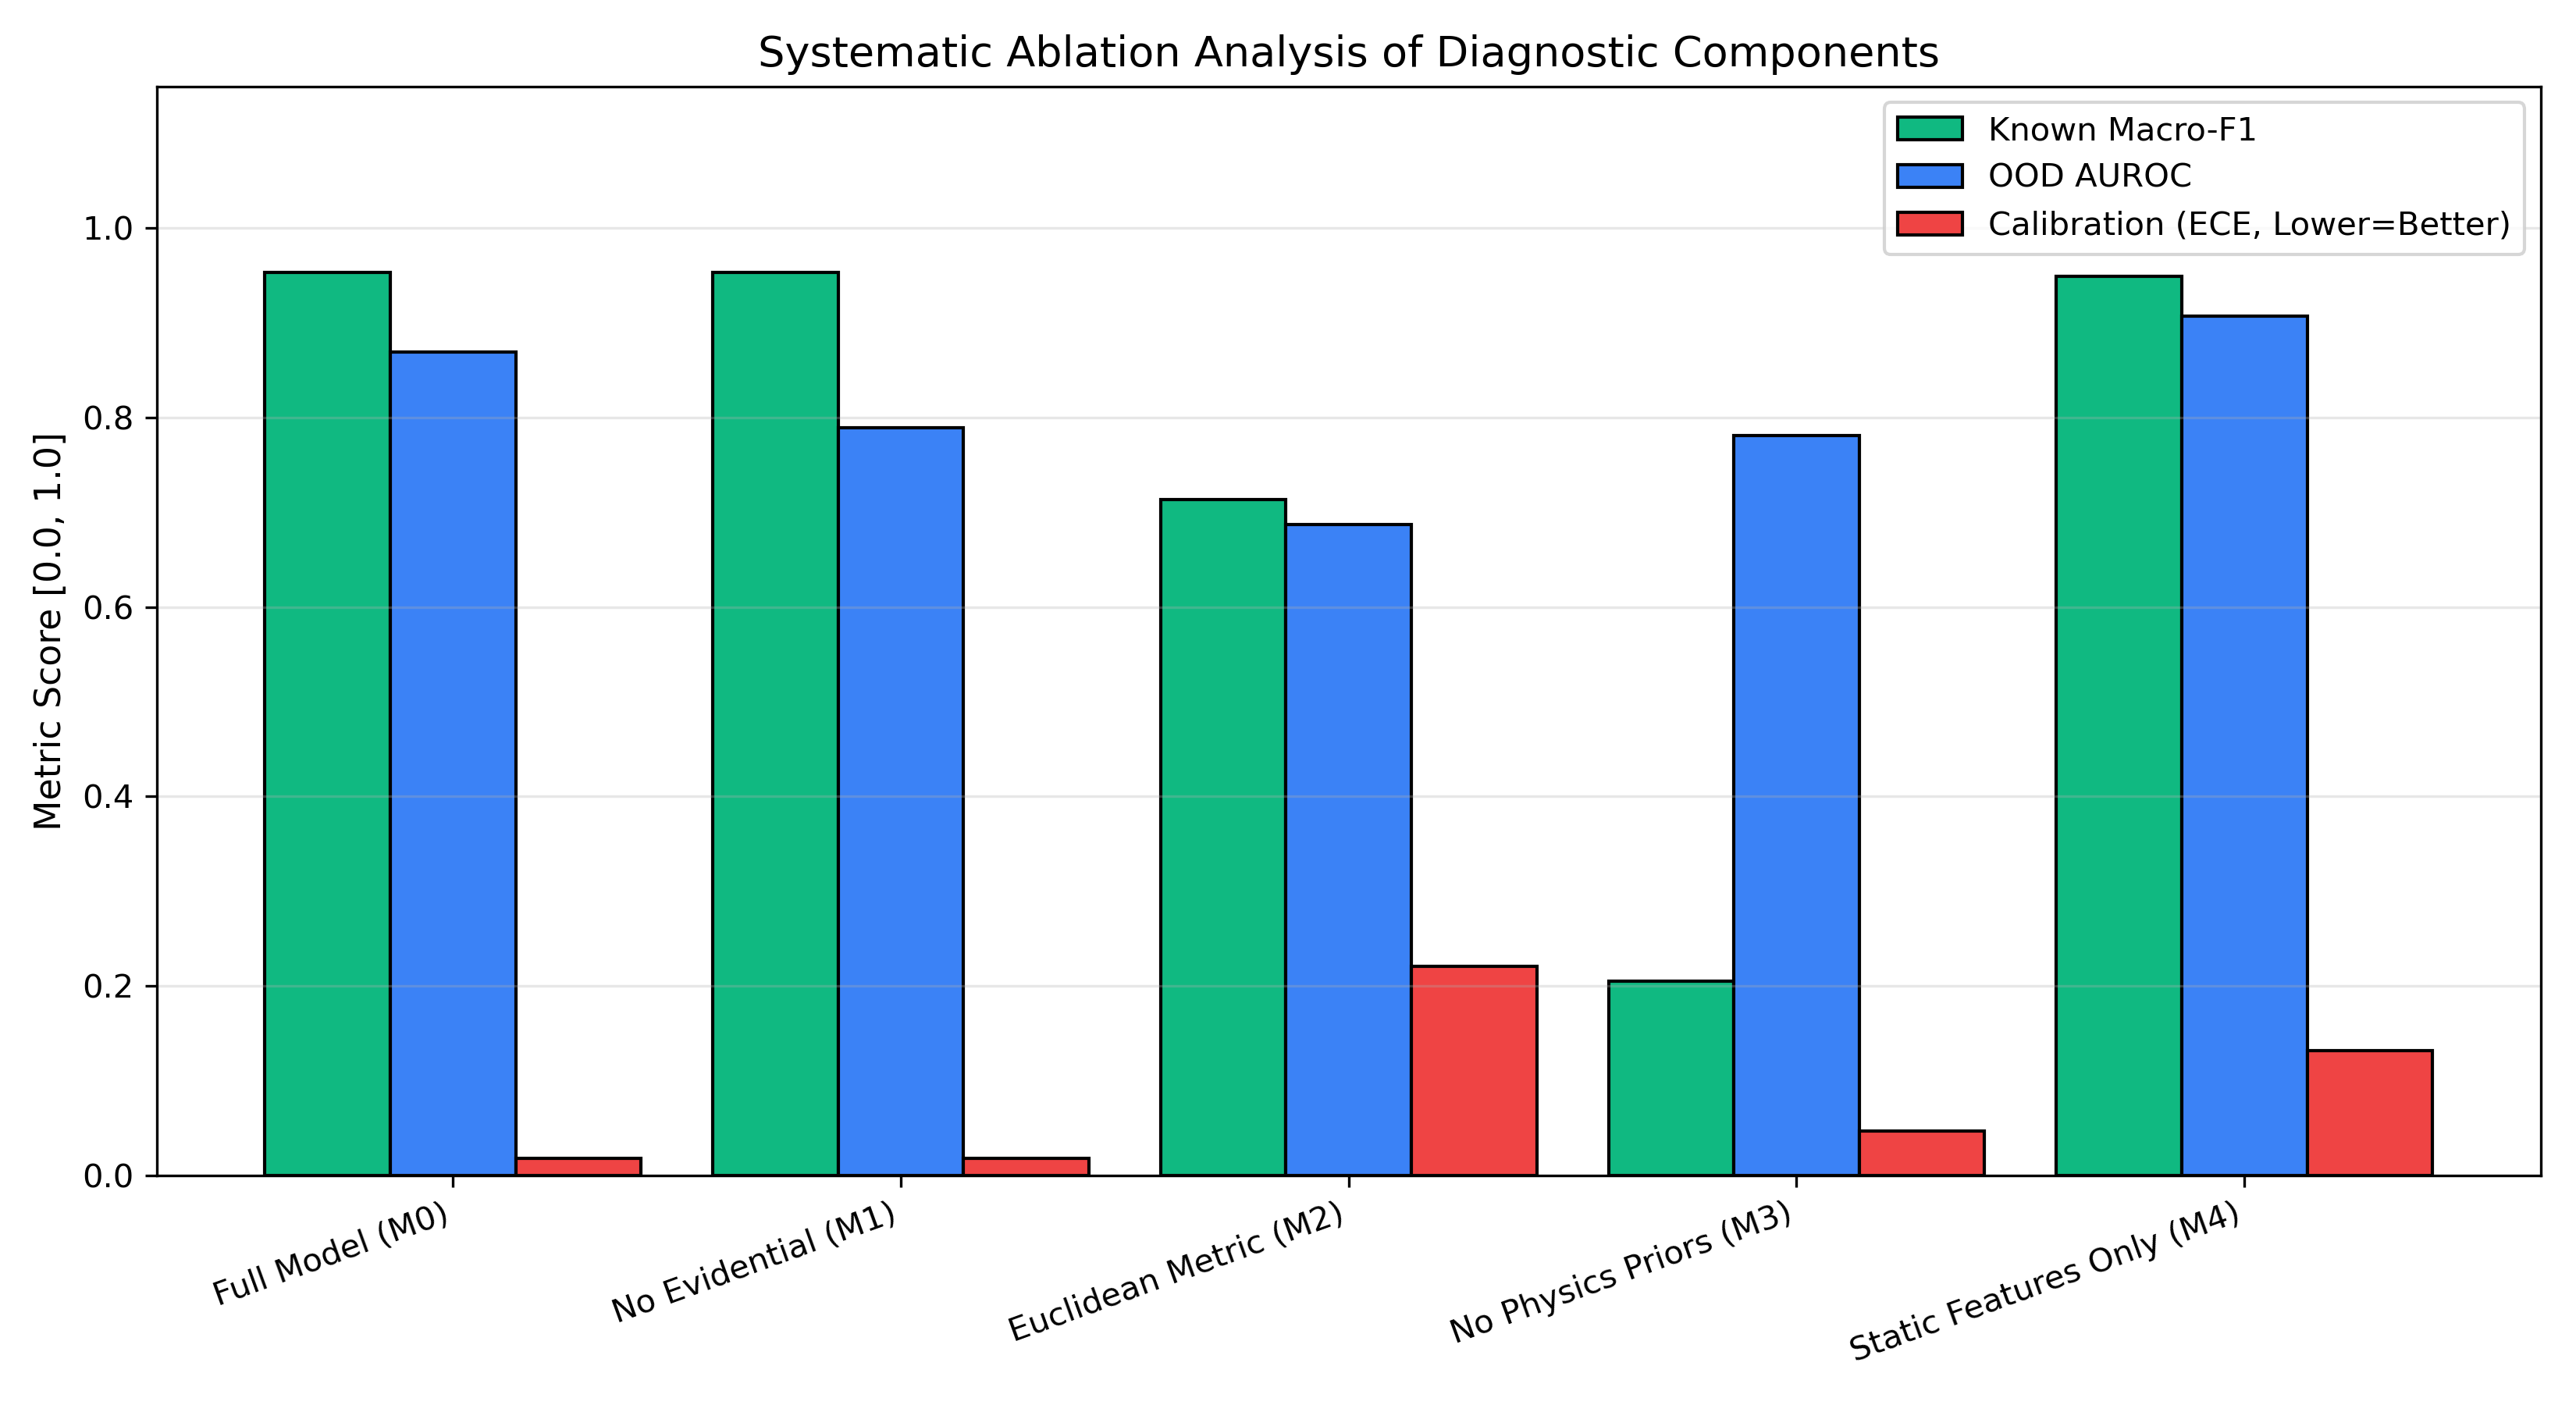
\includegraphics[width=\columnwidth]{figures/fig8_ablation_comparison.png}
\caption{Quantitative ablation comparison across Diagnostic Macro-F1, OOD AUROC, and Expected Calibration Error (ECE) for configurations M0 through M4.}
\label{fig:ablation}
\end{figure}

The Euclidean-metric ablation (M2) produced the clearest degradation in internal-resistance-spike detection, reducing its F1 score to zero. This indicates that the covariance-aware Mahalanobis geometry is important for capturing relationships among the telemetry channels.

Removing the evidential component (M1) reduced OOD AUROC from 0.8692 to 0.7895 in the ablation configuration, a decrease of approximately 8 percentage points. Removing the physics priors (M3) caused a much larger drop in known-fault Macro-F1, to 0.2047. Static features (M4) preserved most of the classification performance but substantially worsened calibration.

\section{Identified Failure Modes and Limitations}

The experiments also reveal boundaries that should be considered before using the method in a flight-critical setting.

\subsection{Compound-Fault Centroid Cancellation}

When two failures occur simultaneously, their effects on different telemetry channels can point in opposing directions. In the tested solar-loss plus thermal-surge case, the resulting feature vector can fall into an intermediate region between modeled fault clusters. The measured epistemic uncertainty in this regime was $0.301\pm0.092$. Consequently, the metric representation can underestimate the unfamiliarity of some compound faults.

\subsection{Magnitude-Invariance Blind Spot}

The use of magnitude-based current features can remove the sign information needed to recognize a polarity reversal. In the sensor sign-inversion experiment, the upstream transformation based on $|I_{\mathrm{batt}}|$ masked the reversal and reduced the catch rate to 6.7\%.

These limitations suggest two direct directions for future work: explicitly preserving signed telemetry features and introducing compound-fault training or structured multi-fault representations.

\section{Conclusion}

This paper evaluated an evidential Dirichlet approach for uncertainty-aware fault diagnosis in autonomous spacecraft health management. The method combines physically motivated telemetry representations with a covariance-aware distance measure and an evidential output layer. The resulting model provides both a diagnosis over known operational modes and an uncertainty signal intended to identify observations that do not belong to the known operating manifold.

On the reported held-out benchmark, the system achieved a Macro-F1 of 0.9533 and an ECE of 0.0094. Telemetry noise primarily increased aleatoric uncertainty, while novel failure conditions produced a large epistemic response. The resulting OOD detector reached an AUROC of 0.9422 and an AUPRC of 0.9516, substantially outperforming the evaluated MSP baseline.

At the same time, the experiments show that uncertainty estimation does not remove the need for careful feature engineering and physical modeling. Compound faults can produce metric cancellation, while magnitude-only representations can hide polarity changes. These failure boundaries are therefore part of the contribution of the study: an uncertainty-aware diagnostic architecture should be evaluated not only by its successful cases, but also by the physical situations in which its assumptions break down.

Future versions of AstraHeal should preserve signed sensor information, support explicit compound-fault hypotheses, and evaluate the uncertainty gating mechanism on broader spacecraft telemetry and independently generated fault scenarios.

\bibliographystyle{IEEEtran}
\bibliography{references}

\end{document}
